\documentclass[border=4pt]{standalone}
\usepackage{tikz}
\begin{document}

\noindent
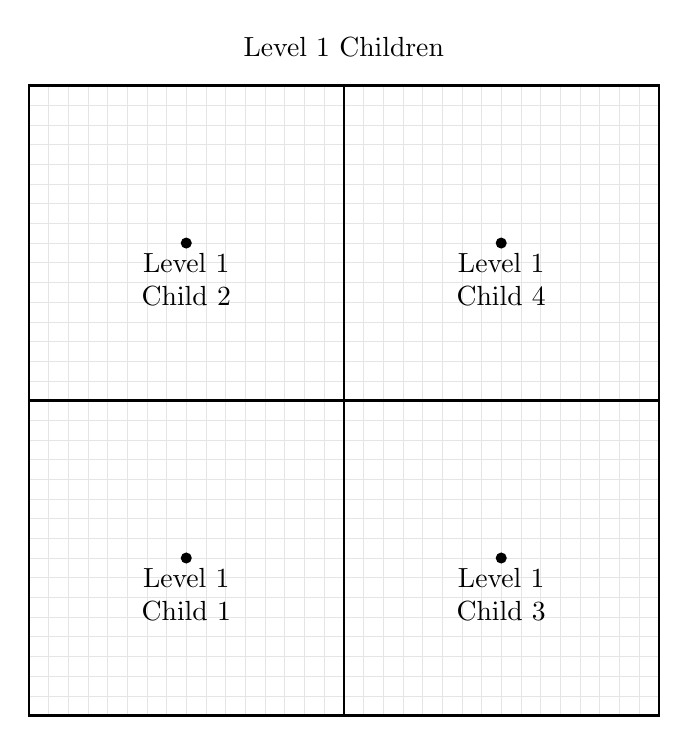
\begin{tikzpicture}[x=0.25cm,y=0.25cm]

  \draw[step=1,black!10,very thin] (0.0,0.0) grid (32.0,32.0);
  \node (TOPL) at (16,33) [above,align=center]  {Level 1 Children};

  \draw[thick] (0,0) rectangle (32,32);

  \draw[thick] (0,0) rectangle (16,16);
  \fill (8,8) circle(2pt);
  \node (0808) at (8,8) [below,align=center]  {Level 1\\Child 1};

  \draw[thick] (0,16) rectangle (16,32); 
  \fill (8,24) circle(2pt);  
  \node (0824) at (8,24) [below,align=center]  {Level 1\\Child 2};

  \draw[thick] (16,0) rectangle (32,16);
  \fill (24,8) circle(2pt);  
  \node (2408) at (24,8) [below,align=center]  {Level 1\\Child 3};

  \draw[thick] (16,16) rectangle (32,32);
  \fill (24,24) circle(2pt);  
  \node (1616) at (24,24) [below,align=center]  {Level 1\\Child 4};

\end{tikzpicture}

\end{document}




